{\fontsize{12}{14}\selectfont 
\begin{figure}[H]
  \centering
  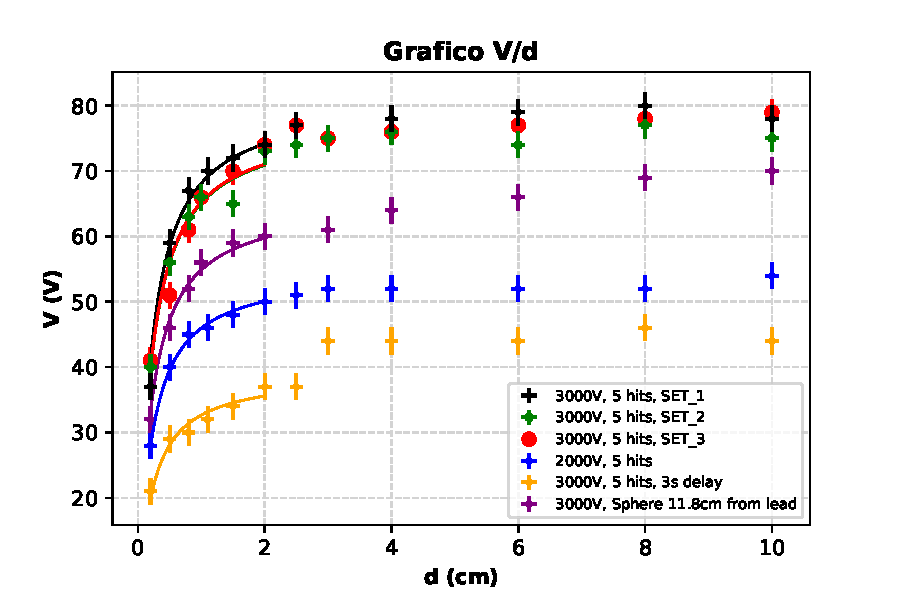
\includegraphics[width=14.5cm]{Figures/Grafico_Parte1.pdf}
  \caption{Grafico della tensione (in Volt) in funzione della distanza (in metri) per sei set differenti. L'errore sulla tensione è pari a $2 V$ mentre quella sulla distanza è di $1 mm$ ovvero il doppio dell'errore di lettura, in quanto presente un errore nella misura della posizione di entrambe le facce del condensatore. Il fit si adatta bene ai dati solo fino a $d = 2 cm$, ovvero in approssimazione $d \ll \sqrt{A} = 15.8 cm$ e non può essere applicato in assenza di questa condizione. Superati i $4cm$ la tensione misurata tende ad un valore di saturazione a causa della capacità del sistema. Si nota inoltre una ripetibilità nei primi 3 set, che sono stati effettuati nelle stesse condizioni.}
  \label{fig:GraficoParteI}
\end{figure}

\begin{figure}[H]
  \centering
  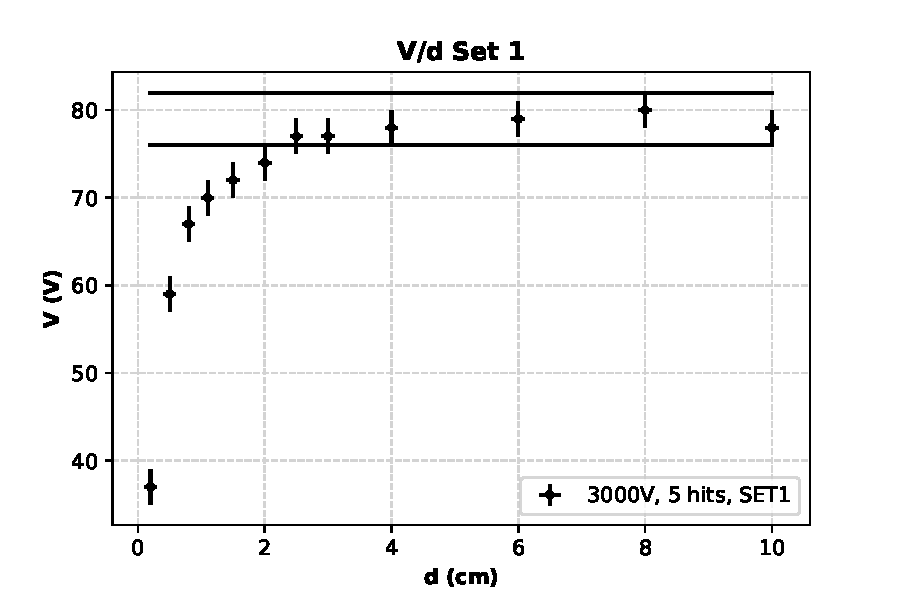
\includegraphics[width=11.5cm]{Figures/Grafico_Parte1_SET1.pdf}
  \caption{Grafico della tensione (in Volt) in funzione della distanza (in metri) per il set 1. Le rette asintotiche sono state tracciate in modo da contenere gli ultimi 3 punti per i quali la capacità del condensatore diventa trascurabile, ponendo quindi in buona approssimazione $V = \dfrac{Q}{C_{sistema}}$}
  \label{fig:parteIset1}
\end{figure}

Per stimare la carica totale $Q$ trasferita al condensatore si considera la sua capacità trascurabile rispetto a $C_{sistema}$ quando la distanza $d \geq 6 cm$, quindi sono state tracciate due rette asintotiche contenenti questi punti come mostrato nel grafico \ref{fig:parteIset1}. Da queste, facendone la semisomma e la semidifferenza si è trovato, per ogni set, il valore di carica presente sul condensatore ed il corrispondente errore.

\begin{align*}
    Q_1 &= (89 \pm 3) 10^{-10} C    &   Q_3 &= (88 \pm 3) 10^{-10} C    &    Q_5 &= (50 \pm 4) 10^{-10} C\\
    Q_2 &= (85 \pm 4) 10^{-10} C    &   Q_4 &= (60 \pm 3) 10^{-10} C    &    Q_6 &= (77 \pm 5) 10^{-10} C
\end{align*}

È stato anche effettuato il calcolo della carica come $Q = (C_{sistema} + C) \cdot V$ per poi fare una media ed una deviazione standard di tutte le misure ottenendo dei valori compatibili con quelli calcolati graficamente.

\begin{align*}
    Q_1 &= (91 \pm 3) 10^{-10} C    &   Q_3 &= (89 \pm 3) 10^{-10} C    &    Q_5 &= (48 \pm 4) 10^{-10} C\\
    Q_2 &= (88 \pm 2) 10^{-10} C    &   Q_4 &= (61.9 \pm 0.9) 10^{-10} C    &    Q_6 &= (75 \pm 3) 10^{-10} C
\end{align*}

Intersecando le barre di errore dei due risultati si sono ottenuti i valori finali di:

\begin{align*}
    Q_1 &= (90 \pm 2) 10^{-10} C    &   Q_3 &= (88.5 \pm 2.5) 10^{-10} C    &    Q_5 &= (49 \pm 3) 10^{-10} C\\
    Q_2 &= (87.5 \pm 1.5) 10^{-10} C    &   Q_4 &= (62 \pm 2) 10^{-10} C    &    Q_6 &= (75 \pm 3) 10^{-10} C
\end{align*}

In particolare la carica presente nei primi 3 set risulta compatibile anche con la carica del quarto set dopo aver moltiplicato il suo valore per $\dfrac{3}{2}$, numero ottenuto dal rapporto delle tensioni a cui era sottoposta la sfera.

\begin{equation*}
    Q_4 \cdot \dfrac{3}{2} = (90 \pm 5) 10^{-10} C 
\end{equation*}

I primi 3 set, ripetuti nelle stesse condizioni, risultano avere una carica compatibile. Intersecando le barre di errore si è quindi ottenuto il risultato finale di:

\begin{equation*}
    Q_{123} = (87.5 \pm 1.5) 10^{-10} C 
\end{equation*}
\par}